
\mode<presentation>
{
  \usetheme{CambridgeUS}
  \usecolortheme{whale}
  \usecolortheme{lily}

  \setbeamercovered{transparent}
  \usefonttheme[onlymath]{serif}
}

\title[\PIDControlDesignShortName] % (optional, use only with long paper titles)
{\course: \PIDControlDesignName\license}

\subtitle
{Lecture \PIDControlDesignNumber} % (optional)


\begin{document}

\begin{frame}
  \titlepage
\end{frame}

\mode<article>{
\maketitle
\tableofcontents
}


\section{Pre-requisite Material}
This lecture assumes that the reader is familiar with the following material:
\begin{itemize}
\item Lecture \ControlAndStabilityNumber:~\ControlAndStabilityName
\item Lecture \HigherOrderResponseNumber:~\HigherOrderResponseName
\item Lecture \PDControlTransientNumber:~\PDControlTransientName
\item Lecture \RotationalAndFluidSystemsNumber:~\RotationalAndFluidSystemsName
\end{itemize}

%%%KEJ note: this "Intro to PID" is now in Lecture 13 (PD control design)
%\section{Intro to PID}
%
%In this lecture, we look at the design of a simple feedback control system. The control will be restricted to have specific terms: a proportional gain, an integral, or a derivative. Using the first initials of the three terms, this is often called a PID controller. This PID control works well for systems that are first or second order (or have dominant dynamics that are first or second order). There are many examples of such systems, thus the PID controller is very common. 
%
%In {\em open loop} (i.e. before we attach a controller) the system to be controlled looks like the following:
%\begin{frame}
%\begin{center}
%\begin{tikzpicture}[scale=1,inner sep=0pt,outer sep=0pt,very thick,
%sysblock/.style={draw,rectangle,inner sep=2pt,minimum width=1.5cm,minimum height=1.25cm,very thick}]
%
%\draw (7,0) node[draw,circle] (sum2) {$\rule{0pt}{18pt}$};
%\draw (9,0) node[sysblock] (G) {$G(s)$};
%
%\draw[->] (5.5,0) node[above=2pt] {$X(s)$}  -- (sum2.180) node[above left=2pt] {$+$};
%\draw[->] (sum2.0) -- (G);
%\draw[->] (G) -- ++(2,0) node[above=2pt] {$Y(s)$};
%\draw[<-] (sum2.90) node[above right=2pt] {$+$} -- ++(0,1) node[right=2pt] {$D(s)$};
%\end{tikzpicture}
%\end{center}
%\begin{itemize}
%\item $G(s)$ - system to be controlled
%\item $D(s)$ - disturbance modeled as input disturbance
%\item $X(s)$ - actuator command
%\item $Y(s)$ - output to be regulated
%\end{itemize}
%\end{frame}
\section{Overview of PID Control}
Proportional, integral, derivative (PID) control is one of the most common types to appear in industry because it is fairly easy to implement and tune. In Lectures~\ControlAndStabilityNumber~and \PDControlTransientNumber, we have seen some examples of P and PD control. In this lecture, we'll do another example of P control for a fluid system, then show how using PI control can improve the steady-state behavior. 

Because PID control can be so commonly used, including in other classes, in the Appendix we provide information about implementing it on a microcontroller. 

\section{Proportional Control}
%\textcolor{red}{the steps 1-3 and mass-spring-damper basic example appear in Lecture 13 (example not identical), but I should repeat some of this P control that deals with steady-state error here, as well, and also the tank height control example}
We have already seen an example of P control for a mass-spring-damper system in Lecture~\PDControlTransientNumber:~\PDControlTransientName. Let's revisit some of the main points, as well as applying this control strategy to a fluid system and then a more generalized mass-spring-damper system. 

\mode<all>{
\mode<article>{To apply feedback control, the output $y$ is measured, compared to a desired reference $r$ to give the error signal $e=r-y$. This error is then applied to the control algorithm. If we use a proportional controller (P), the actuator command $x$ is proportional to the error. The gain of the proportional control will be denoted $K_{p}$. }

\begin{frame}{Proportional Control}
\begin{center}
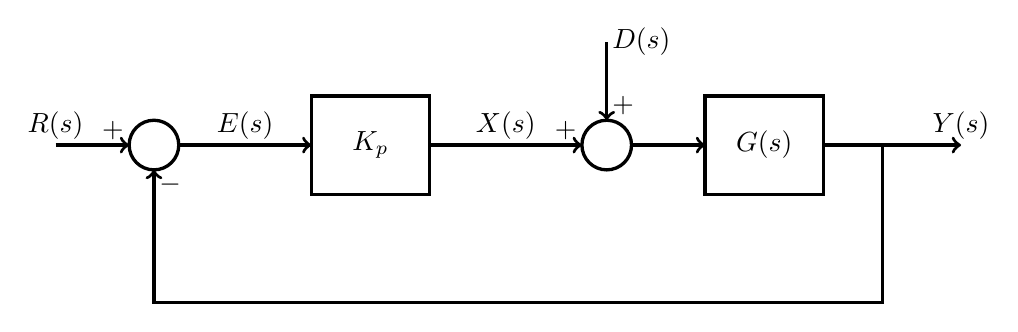
\begin{tikzpicture}[scale=1,inner sep=0pt,outer sep=0pt,very thick,
sysblock/.style={draw,rectangle,inner sep=2pt,minimum width=1.5cm,minimum height=1.25cm,very thick}]

\draw (1.25,0) node[draw,circle] (sum1) {$\rule{0pt}{18pt}$};
\draw (4,0) node[sysblock] (Kp) {$K_{p}$};
\draw (7,0) node[draw,circle] (sum2) {$\rule{0pt}{18pt}$};
\draw (9,0) node[sysblock] (G) {$G(s)$};

\draw[->] (0,0) node[above=2pt] {$R(s)$} -- (sum1.180) node[above left=2pt] {$+$};
\draw[->] (sum1.0) --  node[above=2pt,pos=.5] {$E(s)$} (Kp);
\draw[->] (Kp) -- node[above=2pt,pos=.5] {$X(s)$} (sum2.180) node[above left=2pt] {$+$};
\draw[->] (sum2.0) -- (G);
\draw[->] (G) -- ++(2.5,0) node[above=2pt] {$Y(s)$};
\draw[->] (G) ++(1.5,0) -- ++(0,-2) -| (sum1.-90) node[below right=2pt] {$-$};
\draw[<-] (sum2.90) node[above right=2pt] {$+$} -- ++(0,1) node[right=2pt] {$D(s)$};
\end{tikzpicture}
\end{center}
\end{frame}

When $G(s)$ is a first or second order system, the design of the controller can be straightforward, consisting of three main steps. 
\begin{frame}
\begin{enumerate}
\item \textbf{Collect the design specifications.} Design specifications could be in terms of transient response (rise time, settling time, overshoot) or steady state response (reference tracking or disturbance rejection). 
\item \textbf{Find the relevant {\em closed loop} transfer functions for your design specifications.} \mode<article>{The closed loop transfer functions give the response of the controlled system, as viewed from a reference or disturbance to the output or error. Specifically, using the block diagram simplification rules,}
\begin{align*}
\frac{Y(s)}{R(s)} &= \frac{K_{p}G(s)}{1+K_{p}G(s)}, \\
\frac{E(s)}{R(s)} &= \frac{1}{1+K_{p}G(s)}, \\
\frac{E(s)}{D(s)} &= -\frac{G(s)}{1+K_{p}G(s)}.
\end{align*}
\mode<article>{You will plug the specific open loop transfer function $G(s)$ into these formulas. Note that $\frac{E(s)}{D(s)}$ is only necessary if a disturbance rejection specification is given.}
\item \textbf{Select $K_{p}$ so that the design specifications are met, or determine that no $K_{p}$ exists to meet the specifications.}
\end{enumerate}
\end{frame}

\begin{example}
Design a feedback control system to regulate the height of fluid in a tank, assuming the input flow can be freely assigned. The control system must ensure that the actual tank height follows a reference step command with a settling time $t_{s}\leq 0.2$ s.  In addition, the steady state error between the reference and actual height for a unit step command should be less than or equal to $0.1$. 

A diagram of the feedback control system is below. Note that the output $y$ is the measurement of the tank height $h$. This is subtracted from the reference $r$. The resulting error is multiplied by $K_{p}$ and the flow is set to be this value. The area of the tank is $2$ square meters, the valve constant is $9.81/4$, and the fluid density is $\rho=1$.  

\begin{frame}
\begin{center}
\begin{tikzpicture}
\draw (.75,0) node[above] (tank) {\input{\mainfolder/DrawingElements/FluidElements/tank.tex}};
\draw[decorate,decoration={coil,aspect=0,segment length=5.85pt}] (-.45,2.25) -- ++(2.38,0);
\draw (-1.15,1) node (pipe1) {\input{\mainfolder/DrawingElements/FluidElements/pipe.tex}};
\draw (2.65,1) node (pipe2) {\input{\mainfolder/DrawingElements/FluidElements/valve.tex}};

\draw (1.7,3) node[inner sep=0,outer sep=0] (meas) {\begin{tikzpicture} \draw[very thick] (0,0) -- ++(.1,0) -- ++(0,-.1) -- ++(.2,0) -- ++(0,.1) -- ++(.1,0) -- ++(0,.4) -- ++(-.4,0) -- cycle;\end{tikzpicture}};
\draw (-5.75,1) node[draw,circle,very thick] (sum) {\rule{9pt}{0pt}};
\draw (-4,1) node[draw,rectangle,very thick,minimum width=.5in,minimum height=.5in,outer sep=0pt] (C) {$K_{p}$};

\draw[->,thick,dotted] (meas.90) -- ++(0,.3) node[above left] {measurement of $y=h$} -| (sum.90) node[above right] {$-$};
\draw[<-,thick,dotted] (sum.180) node[above left] {$+$} -- ++(-1,0) node[above] {$r$};
\draw[->,thick,dotted] (sum.0) -- (C.180);
\draw[->,thick,dotted] (C.0) -- ++(.65,0);



\draw[->] (.2,.75) -- node[pos=.5,left] {$h$} ++(0,1.4);
\draw (tank.-90) node{Tank Area: $2$ m$^{2}$};
\draw (pipe2.90) node[above] {$\frac{9.81}{4}$};
\draw (.75,.8) node[above] {$p_{1}$};
\draw[<-] (pipe1.180) ++(.9,0) --  ++(-.5,0) node[left=5pt] {$x=q_{in}$};
\draw[->] (pipe2.0) ++(-.5,0) --  ++(.5,0) node[right] {$q_{out}$};
\draw (.75,2.5) node[above] {$p_{a}$};
\draw (pipe2.0) ++(1.5,0) node {$p_{a}$};
\end{tikzpicture}
\end{center}
\end{frame}

The open loop system transfer function is found using our standard modeling techniques. For example, the following expresses the system as an impedance network with the reference at atmospheric pressure $p_{a}$.

\begin{frame}
\begin{center}
\begin{tikzpicture}
\draw (-2,-1.5) node[scale=.85,inner sep=0pt,outer sep=0pt] (a) {\input{\mainfolder/DrawingElements/CircuitElements/currentsource.tex}};
\draw (-.5,0) node[circle,fill=black,inner sep=0,minimum width=4pt] {} node[above=4pt,circle, inner sep=1pt,fill=yellow] {$P_{1}$};
\draw (a) node[left=9pt] {$Q_{in}(s)$};
\draw (-.5,-1.5) node[rectangle,draw,minimum width=.1in,minimum height=.5in] (tank1) {};
\draw (tank1) node[right=9pt] {$\frac{\rho g}{sA_{1}}$};
\draw (1,0) node[rectangle,draw,minimum width=.5in,minimum height=.1in] (valve1) {};
\draw (valve1) node[above=9pt] {$R_{1}$};
\draw (2.5,-3) node[inner sep=0] (pa) {};
\draw (-.5,-3) node[circle,fill=black,minimum width=4pt,inner sep=0] {};
\draw (-.5,-3) node[below=4pt,circle, inner sep=1pt,fill=pink] {$P_{a}$};
\draw (2.5,-3) node[inner sep=0,outer sep=0] (pa2) {};
\draw (-.5,-3) node[inner sep=0,outer sep=0] (pa3) {};
\draw[very thick] (a.90) |- (valve1.180);
\draw[very thick] (tank1.90) |- (valve1.180);
\draw[very thick] (valve1.0) -| (pa) -- (pa3);
\draw[very thick] (tank1.-90) -- (pa3) -| (a.-90);
\draw[->] (3,-1) -- node[pos=.5,right] {$Q_{out}(s)$} ++(0,-1);
\end{tikzpicture}
\mode<presentation>{\[
\frac{Q_{out}(s)}{Q_{in}(s)} = \frac{\frac{1}{2}}{s+2}
\]}
\end{center}
\end{frame}
We also have the auxiliary equation $\rho g h = p_{1}$, or since $\rho=1$, $h=\frac{1}{g}p_{1}$. Thus, the transfer function $H(s)/Q_{in}(s)$ can be found by first finding $P_{1}/Q_{in}(s)$, and then dividing by $g$. Combining the impedances in parallel, 
\begin{align*}
\frac{P_{1}}{Q_{in}(s)}&= \frac{\frac{g}{2s}\frac{9.81}{4}}{\frac{g}{2s} + \frac{9.81}{4}} \\
 &= \frac{\frac{g}{2}}{\frac{2g}{9.81} + s} 
\end{align*}
Using $g=9.81$ and $h=\frac{1}{g}p_{1}$
\[
G(s) = \frac{H(s)}{Q_{in}(s)} = \frac{\frac{1}{2}}{s+2}
\]

The feedback control system can be represented with the following block diagram. (Since no disturbance rejection specification was listed, a disturbance input was not included.) Note that $R(s)$ is the {\em desired} tank height.

\begin{frame}
\begin{center}
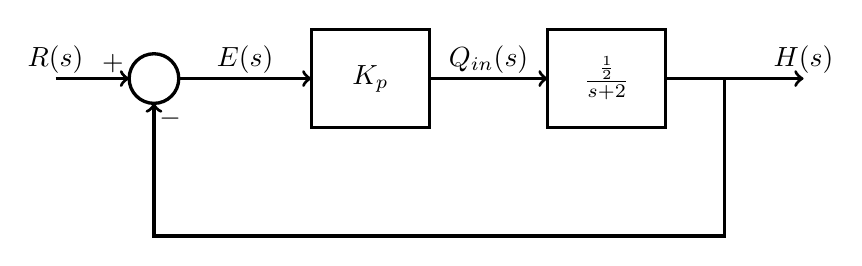
\begin{tikzpicture}[scale=1,inner sep=0pt,outer sep=0pt,very thick,
sysblock/.style={draw,rectangle,inner sep=2pt,minimum width=1.5cm,minimum height=1.25cm,very thick}]

\draw (1.25,0) node[draw,circle] (sum1) {$\rule{0pt}{18pt}$};
\draw (4,0) node[sysblock] (Kp) {$K_{p}$};
\draw (7,0) node[sysblock] (G) {$\frac{\frac{1}{2}}{s+2}$};

\draw[->] (0,0) node[above=2pt] {$R(s)$} -- (sum1.180) node[above left=2pt] {$+$};
\draw[->] (sum1.0) --  node[above=2pt,pos=.5] {$E(s)$} (Kp);
\draw[->] (Kp) -- node[above=2pt] {$Q_{in}(s)$} (G);
\draw[->] (G) -- ++(2.5,0) node[above=2pt] {$H(s)$};
\draw[->] (G) ++(1.5,0) -- ++(0,-2) -| (sum1.-90) node[below right=2pt] {$-$};
\end{tikzpicture}
\end{center}
\end{frame}

We can now proceed with the design process:

\begin{frame}
\begin{enumerate}
\item Design specifications
\begin{itemize}
\item $\ts \leq 0.2$ s
\item $e_{ss}\leq 0.1$ for unit step reference
\end{itemize}
\item Closed loop transfer functions
\begin{align*}
\frac{H(s)}{R(s)} &= \frac{K_{p}/2}{s+\frac{K_{p}}{2}+2}\\
\frac{E(s)}{R(s)} &= \frac{s+2}{s+\frac{K_{p}}{2}+2}\\ 
\end{align*}
Note that the closed loop transfer functions are also first order.
\end{enumerate}
\end{frame}
\begin{frame}
\mode<presentation>{
\begin{center}
$\frac{H(s)}{R(s)} = \frac{K_{p}/2}{s+\frac{K_{p}}{2}+2} \quad \frac{E(s)}{R(s)} = \frac{s+2}{s+\frac{K_{p}}{2}+2}$
\end{center}
}
\begin{enumerate}
\setcounter{enumi}{1}
\item Select $K_{p}$. 
\mode<presentation>{
\begin{itemize}
\item<2-> $\ts \leq 0.2$. 
\[
\ts = \tseqone \leq 0.2 \implies \sigma \geq \frac{4.6}{0.2} = 23
\]
\[
\uncover<3->{\sigma = \frac{K_{p}}{2}+2 \geq 23 \implies K_{p} \geq 42}
\]
\item<4-> $e_{ss}\leq 0.1$.
\[
e_{ss} = \lim_{s\rightarrow 0} s E(s) = \lim_{s\rightarrow 0} s \frac{E(s)}{R(s)}\frac{1}{s} =  s\frac{s+2}{s+\frac{K_{p}}{2}+2}\frac{1}{s} = \frac{2}{2+\frac{K_{p}}{2}} 
\]
\[
\uncover<5->{e_{ss}= \frac{2}{2+\frac{K_{p}}{2}} \leq 0.1 \implies K_{p} \geq 36}
\]
\end{itemize}
}
\mode<article>{We have two specifications. The first constraint on settling time can be converted to a constraint on the closed loop pole location. We previously showed that for a first order system with pole at $s=-\sigma$,
\[
\ts = \tseqone
\]
Since our specification is $t_{s}\leq 0.2$, we require $\frac{4.6}{\sigma}\leq 0.2$ or
\[
\sigma \geq \frac{4.6}{0.2} = 23
\]
The pole of our closed loop feedback system is at $s=-(\frac{K_{p}}{2}+2)$. Thus, we need to choose
\[
\frac{K_{p}}{2}+2 \geq 23
\]
or
\[
K_{p} \geq 42.
\]
The second constraint on reference steady state error translates to a constraint on the DC gain of $K_{p}G(s)$. We can either recall that for a step reference $e_{ss}=\frac{1}{1+K_{s}}$ where $K_{s} = K_{p}G(0) = \frac{K_{p}}{4}$, or we can solve directly using the final value theorem
\[
e_{ss} = \lim_{s\rightarrow 0} s E(s) = \lim_{s\rightarrow 0} s \frac{s+2}{s+\frac{K_{p}}{2}+2}\frac{1}{s} = \frac{2}{2+\frac{K_{p}}{2}} =\frac{1}{1+\frac{K_{p}}{4}}
\]
Since we require
\[
e_{ss} = \frac{1}{1+\frac{K_{p}}{4}} \leq 0.1,
\]
we can solve for the constraint
\[
K_{p} \geq 36
\]
Since the most stringent requirement is on the settling time, our final design choice is
\[
\boxed{K_{p} \geq 42}
\]}
\end{enumerate}
\end{frame}

\end{example}


\begin{example} Determine how a proportional feedback control system will change the closed loop behavior when controlling the position of the mass-spring-damper system using force actuation
\begin{frame}
\begin{center}
\begin{tikzpicture}[scale=1.75,inner sep=0pt,outer sep=0pt,very thick]
\draw (.3,0) node[fill] (a) {}; 
\draw (1.7,0) node[fill] (b) {};
 
\draw (0,0) node (gnd1) {\input{\mainfolder/DrawingElements/MechanicalElements/ground.tex}};
\draw (1,.3) node (K1) {\begin{tikzpicture}
\draw (.75,0) node[inner sep=0,outer sep=0] (K1) {\begin{tikzpicture}
\draw (.75,0) node[inner sep=0,outer sep=0] (K1) {\input{\mainfolder/DrawingElements/MechanicalElements/spring.tex}};
\draw (K1)  node[above=6pt] {$k$};
\draw[very thick] (K1.180) -- ++(-.2,0);
\draw[very thick] (K1.0) -- ++(0.2,0);
\draw[<-,thick] (K1.0) ++(.2,0) -- ++(.5,0) node[right] {$f$};
\draw[<-,thick] (K1.180) ++(-.2,0) -- ++(-.5,0) node[left] {$f$};
\draw[|->,thick] (K1.180) ++(-.2,.4) node[above=2pt] {$x_{1}$} -- ++(.5,0);  
\draw[|->,thick] (K1.0) ++(.2,.4) node[above=2pt] {$x_{2}$} -- ++(.5,0);  
\draw<2-> (K1) ++(0,-.6) node {$f=k(x_{1}-x_{2})$};
\end{tikzpicture}
};
\draw (K1)  node[above=6pt] {$k$};
\draw[very thick] (K1.180) -- ++(-.2,0);
\draw[very thick] (K1.0) -- ++(0.2,0);
\draw[<-,thick] (K1.0) ++(.2,0) -- ++(.5,0) node[right] {$f$};
\draw[<-,thick] (K1.180) ++(-.2,0) -- ++(-.5,0) node[left] {$f$};
\draw[|->,thick] (K1.180) ++(-.2,.4) node[above=2pt] {$x_{1}$} -- ++(.5,0);  
\draw[|->,thick] (K1.0) ++(.2,.4) node[above=2pt] {$x_{2}$} -- ++(.5,0);  
\draw<2-> (K1) ++(0,-.6) node {$f=k(x_{1}-x_{2})$};
\end{tikzpicture}
};
\draw (1,.3) node[above=.2in] {$k$};
\draw (1,-.3) node (D) {\begin{tikzpicture}
\draw[very thick] (-.2,0) -- (0,0);
\draw (.75,0) node {\begin{tikzpicture}
\draw[very thick] (-.2,0) -- (0,0);
\draw (.75,0) node {\input{\mainfolder/DrawingElements/MechanicalElements/damper.tex}};
\draw (.75,0) node[above=9pt] {$b$};
\draw[very thick] (1.5,0) -- ++(.2,0);
    \draw[<-,thick] (1.5,0) ++(.2,0) -- ++(.5,0) node[right] {$f$};
    \draw[<-,thick] (-.2,0) -- ++(-.5,0) node[left] {$f$};
    \draw[|->,thick] (-.2,.4) node[above=2pt] {$x_{1}$} -- ++(.5,0);  
    \draw[|->,thick] (1.7,.4) node[above=2pt] {$x_{2}$} -- ++(.5,0);  
    \draw (.6,-.6) node {$x=x_{1}-x_{2}$};
  %  \draw (.6,-1.2) node {$f=b\dot{x}$};
\end{tikzpicture}};
\draw (.75,0) node[above=9pt] {$b$};
\draw[very thick] (1.5,0) -- ++(.2,0);
    \draw[<-,thick] (1.5,0) ++(.2,0) -- ++(.5,0) node[right] {$f$};
    \draw[<-,thick] (-.2,0) -- ++(-.5,0) node[left] {$f$};
    \draw[|->,thick] (-.2,.4) node[above=2pt] {$x_{1}$} -- ++(.5,0);  
    \draw[|->,thick] (1.7,.4) node[above=2pt] {$x_{2}$} -- ++(.5,0);  
    \draw (.6,-.6) node {$x=x_{1}-x_{2}$};
  %  \draw (.6,-1.2) node {$f=b\dot{x}$};
\end{tikzpicture}};
\draw (1,-.3) node[below=.22in] {$b$};
\draw (2.5,0) node (M1) {\input{\mainfolder/DrawingElements/MechanicalElements/mass2.tex}};
\draw (2.5,0) node {$m$};
\draw[|->] (2.5,.8) node[above=.15in] {$y$} -- ++(.5,0);


\draw (gnd1) -- (a);
\draw (a) |- (K1);
\draw (a) |- (D);
\draw (K1) -| (b);
\draw (D) -| (b);
\draw (b) -- (M1);
%\draw[->] (M1.0) ++(0,.4) -- ++(.5,0) node[right] {$d$};
\draw[->] (M1.0) -- ++(.5,0) node[right] {$f$};

\end{tikzpicture}
\end{center}
\[
\frac{Y(s)}{F(s)} = \frac{1/m}{s^{2}+(b/m)s + (k/m)}
\]
\end{frame}

The proportional feedback control system would be represented by the block diagram
\begin{frame}
\begin{center}
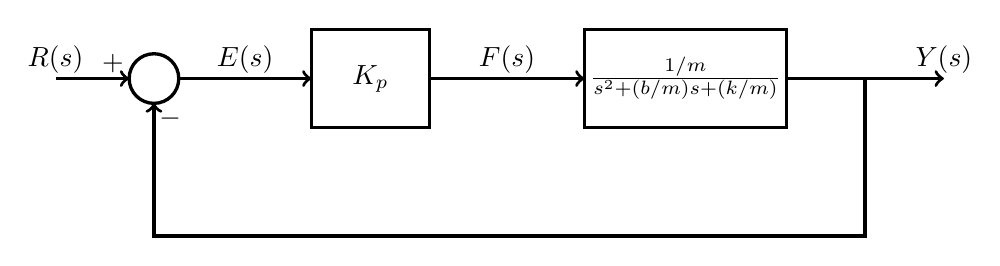
\begin{tikzpicture}[scale=1,inner sep=0pt,outer sep=0pt,very thick,
sysblock/.style={draw,rectangle,inner sep=2pt,minimum width=1.5cm,minimum height=1.25cm,very thick}]

\draw (1.25,0) node[draw,circle] (sum1) {$\rule{0pt}{18pt}$};
\draw (4,0) node[sysblock] (Kp) {$K_{p}$};
\draw (8,0) node[sysblock] (G) {$\frac{1/m}{s^{2}+(b/m)s + (k/m)}$};

\draw[->] (0,0) node[above=2pt] {$R(s)$} -- (sum1.180) node[above left=2pt] {$+$};
\draw[->] (sum1.0) --  node[above=2pt,pos=.5] {$E(s)$} (Kp);
\draw[->] (Kp) -- node[above=2pt, pos=.5] {$F(s)$} (G);
\draw[->] (G.0) -- ++(2,0) node[above=2pt] {$Y(s)$};
\draw[->] (G.0) ++(1,0) -- ++(0,-2) -| (sum1.-90) node[below right=2pt] {$-$};
\end{tikzpicture}
\mode<presentation>{
\[
F(s) = K_{p}(R(s) - Y(s))
\]
\[
f(t) = K_{p}(r(t) - y(t))
\]
}
\end{center}
\end{frame}



The closed loop transfer function is
\begin{frame}
\[
\frac{Y(s)}{R(s)} = \frac{K_{p}/m}{s^{2}+(b/m)s+(k+K_{p})/m}.
\]

\mode<article>{We can get a very general sense of how changes in $K_{p}$ affect the transient response by finding the damping ratio and natural frequency for the closed loop poles. In particular}
\visible<2->{\[\omega_{n} = \sqrt{\frac{k+K_{p}}{m}}, \quad
\zeta  = \frac{b}{2\sqrt{m}\sqrt{k+K_{p}}}, \quad
\zeta\omega_{n}  = \frac{b}{2m}. 
\]}

\mode<article>{From the form of these equations we see that} 
\visible<3->{\begin{align*}
\uparrow K_{p} \implies\begin{cases} \uparrow  \omega_{n} & \implies \mbox{reduced rise time}\\
 \downarrow\zeta & \implies \mbox{increased overshoot} \\
\leftrightarrow \ts & \implies \mbox{no change in settling time} \end{cases}
\end{align*}}
\end{frame}
Thus, while increasing $K_{p}$ makes the response faster, it also makes it more oscillatory, and in the second order case, proportional control cannot change the settling time.

\end{example}

A physical intuition for the behavior of proportional control on a second order system can be obtained by implementing proportional control using a {\em mechanical} controller. Note that in proportional control, the control force $f$ should be given by 
\[
f(t) = K_{p}(r(t)-y(t)).
\]
Let's implement this force by attaching a spring with spring constant $K_{p}$ with one end on the mass, and the other end attached to a point that specifies the reference $r$, as follows:
\begin{frame}
\begin{center}
\begin{tikzpicture}[scale=1.75,inner sep=0pt,outer sep=0pt,very thick]
\draw (.3,0) node[fill] (a) {}; 
\draw (1.7,0) node[fill] (b) {};
 
\draw (0,0) node (gnd1) {\input{\mainfolder/DrawingElements/MechanicalElements/ground.tex}};
\draw (1,.3) node (K1) {\begin{tikzpicture}
\draw (.75,0) node[inner sep=0,outer sep=0] (K1) {\begin{tikzpicture}
\draw (.75,0) node[inner sep=0,outer sep=0] (K1) {\input{\mainfolder/DrawingElements/MechanicalElements/spring.tex}};
\draw (K1)  node[above=6pt] {$k$};
\draw[very thick] (K1.180) -- ++(-.2,0);
\draw[very thick] (K1.0) -- ++(0.2,0);
\draw[<-,thick] (K1.0) ++(.2,0) -- ++(.5,0) node[right] {$f$};
\draw[<-,thick] (K1.180) ++(-.2,0) -- ++(-.5,0) node[left] {$f$};
\draw[|->,thick] (K1.180) ++(-.2,.4) node[above=2pt] {$x_{1}$} -- ++(.5,0);  
\draw[|->,thick] (K1.0) ++(.2,.4) node[above=2pt] {$x_{2}$} -- ++(.5,0);  
\draw<2-> (K1) ++(0,-.6) node {$f=k(x_{1}-x_{2})$};
\end{tikzpicture}
};
\draw (K1)  node[above=6pt] {$k$};
\draw[very thick] (K1.180) -- ++(-.2,0);
\draw[very thick] (K1.0) -- ++(0.2,0);
\draw[<-,thick] (K1.0) ++(.2,0) -- ++(.5,0) node[right] {$f$};
\draw[<-,thick] (K1.180) ++(-.2,0) -- ++(-.5,0) node[left] {$f$};
\draw[|->,thick] (K1.180) ++(-.2,.4) node[above=2pt] {$x_{1}$} -- ++(.5,0);  
\draw[|->,thick] (K1.0) ++(.2,.4) node[above=2pt] {$x_{2}$} -- ++(.5,0);  
\draw<2-> (K1) ++(0,-.6) node {$f=k(x_{1}-x_{2})$};
\end{tikzpicture}
};
\draw (1,.3) node[above=.2in] {$k$};
\draw (1,-.3) node (D) {\begin{tikzpicture}
\draw[very thick] (-.2,0) -- (0,0);
\draw (.75,0) node {\begin{tikzpicture}
\draw[very thick] (-.2,0) -- (0,0);
\draw (.75,0) node {\input{\mainfolder/DrawingElements/MechanicalElements/damper.tex}};
\draw (.75,0) node[above=9pt] {$b$};
\draw[very thick] (1.5,0) -- ++(.2,0);
    \draw[<-,thick] (1.5,0) ++(.2,0) -- ++(.5,0) node[right] {$f$};
    \draw[<-,thick] (-.2,0) -- ++(-.5,0) node[left] {$f$};
    \draw[|->,thick] (-.2,.4) node[above=2pt] {$x_{1}$} -- ++(.5,0);  
    \draw[|->,thick] (1.7,.4) node[above=2pt] {$x_{2}$} -- ++(.5,0);  
    \draw (.6,-.6) node {$x=x_{1}-x_{2}$};
  %  \draw (.6,-1.2) node {$f=b\dot{x}$};
\end{tikzpicture}};
\draw (.75,0) node[above=9pt] {$b$};
\draw[very thick] (1.5,0) -- ++(.2,0);
    \draw[<-,thick] (1.5,0) ++(.2,0) -- ++(.5,0) node[right] {$f$};
    \draw[<-,thick] (-.2,0) -- ++(-.5,0) node[left] {$f$};
    \draw[|->,thick] (-.2,.4) node[above=2pt] {$x_{1}$} -- ++(.5,0);  
    \draw[|->,thick] (1.7,.4) node[above=2pt] {$x_{2}$} -- ++(.5,0);  
    \draw (.6,-.6) node {$x=x_{1}-x_{2}$};
  %  \draw (.6,-1.2) node {$f=b\dot{x}$};
\end{tikzpicture}};
\draw (1,-.3) node[below=.22in] {$b$};
\draw (2.5,0) node (M1) {\input{\mainfolder/DrawingElements/MechanicalElements/mass2.tex}};
\draw (2.5,0) node {$m$};
\draw[|->] (2.5,.8) node[above=.15in] {$y$} -- ++(.5,0);
\draw (4,0) node (K2) {\begin{tikzpicture}
\draw (.75,0) node[inner sep=0,outer sep=0] (K1) {\begin{tikzpicture}
\draw (.75,0) node[inner sep=0,outer sep=0] (K1) {\input{\mainfolder/DrawingElements/MechanicalElements/spring.tex}};
\draw (K1)  node[above=6pt] {$k$};
\draw[very thick] (K1.180) -- ++(-.2,0);
\draw[very thick] (K1.0) -- ++(0.2,0);
\draw[<-,thick] (K1.0) ++(.2,0) -- ++(.5,0) node[right] {$f$};
\draw[<-,thick] (K1.180) ++(-.2,0) -- ++(-.5,0) node[left] {$f$};
\draw[|->,thick] (K1.180) ++(-.2,.4) node[above=2pt] {$x_{1}$} -- ++(.5,0);  
\draw[|->,thick] (K1.0) ++(.2,.4) node[above=2pt] {$x_{2}$} -- ++(.5,0);  
\draw<2-> (K1) ++(0,-.6) node {$f=k(x_{1}-x_{2})$};
\end{tikzpicture}
};
\draw (K1)  node[above=6pt] {$k$};
\draw[very thick] (K1.180) -- ++(-.2,0);
\draw[very thick] (K1.0) -- ++(0.2,0);
\draw[<-,thick] (K1.0) ++(.2,0) -- ++(.5,0) node[right] {$f$};
\draw[<-,thick] (K1.180) ++(-.2,0) -- ++(-.5,0) node[left] {$f$};
\draw[|->,thick] (K1.180) ++(-.2,.4) node[above=2pt] {$x_{1}$} -- ++(.5,0);  
\draw[|->,thick] (K1.0) ++(.2,.4) node[above=2pt] {$x_{2}$} -- ++(.5,0);  
\draw<2-> (K1) ++(0,-.6) node {$f=k(x_{1}-x_{2})$};
\end{tikzpicture}
};
\draw (4,0) node[above=.2in] {$K_p$};


\draw (gnd1) -- (a);
\draw (a) |- (K1);
\draw (a) |- (D);
\draw (K1) -| (b);
\draw (D) -| (b);
\draw (b) -- (M1);
\draw (M1) -- (K2);
\draw[->] (M1.0) ++(0,.4) -- ++(.5,0) node[right] {$d$};
\draw[-o] (K2.0) -- ++(.5,0);
\draw[|->] (K2.0) ++(.42,.2) node[above=.15in] {$r$} -- ++(.5,0);
\end{tikzpicture}
\mode<presentation>{
\[
f(t) = K_{p}(r(t)-y(t))
\]
}
\end{center}
\end{frame}
Increasing $K_{p}$ corresponds to increasing the spring constant. Thus, the system becomes stiffer, but without added damping, this means the response is more oscillatory.

}
Mass-spring-damper systems tend to be underdamped, often requiring D control to dampen oscillations. See Lecture~\PDControlTransientNumber:~\PDControlTransientName~for more information.

%\section{Proportional/Derivative (PD) Control}
%\mode<all>{\textcolor{red}{commented items for mass-spring-damper PD control that have been incorporated into the new PD control lecture in Fa'22}
%\mode<article>{An intuitive fix for the oscillatory response that proportional control can cause is to change our control so that it implements additional damping. Using mechanical components, we could add a damper between ground and the mass.}
%\begin{frame}{Mechanical Proportional/Derivative Control}
%\begin{center}
%\begin{tikzpicture}[scale=1.75,inner sep=0pt,outer sep=0pt,very thick]
%\draw (.3,0) node[fill] (a) {}; 
%\draw (1.7,0) node[fill] (b) {};
%\draw (3.7,0) node[fill] (c) {};
% 
%\draw (0,0) node (gnd1) {\input{\mainfolder/DrawingElements/MechanicalElements/ground.tex}};
%\draw (1,.3) node (K1) {\begin{tikzpicture}
\draw (.75,0) node[inner sep=0,outer sep=0] (K1) {\begin{tikzpicture}
\draw (.75,0) node[inner sep=0,outer sep=0] (K1) {\input{\mainfolder/DrawingElements/MechanicalElements/spring.tex}};
\draw (K1)  node[above=6pt] {$k$};
\draw[very thick] (K1.180) -- ++(-.2,0);
\draw[very thick] (K1.0) -- ++(0.2,0);
\draw[<-,thick] (K1.0) ++(.2,0) -- ++(.5,0) node[right] {$f$};
\draw[<-,thick] (K1.180) ++(-.2,0) -- ++(-.5,0) node[left] {$f$};
\draw[|->,thick] (K1.180) ++(-.2,.4) node[above=2pt] {$x_{1}$} -- ++(.5,0);  
\draw[|->,thick] (K1.0) ++(.2,.4) node[above=2pt] {$x_{2}$} -- ++(.5,0);  
\draw<2-> (K1) ++(0,-.6) node {$f=k(x_{1}-x_{2})$};
\end{tikzpicture}
};
\draw (K1)  node[above=6pt] {$k$};
\draw[very thick] (K1.180) -- ++(-.2,0);
\draw[very thick] (K1.0) -- ++(0.2,0);
\draw[<-,thick] (K1.0) ++(.2,0) -- ++(.5,0) node[right] {$f$};
\draw[<-,thick] (K1.180) ++(-.2,0) -- ++(-.5,0) node[left] {$f$};
\draw[|->,thick] (K1.180) ++(-.2,.4) node[above=2pt] {$x_{1}$} -- ++(.5,0);  
\draw[|->,thick] (K1.0) ++(.2,.4) node[above=2pt] {$x_{2}$} -- ++(.5,0);  
\draw<2-> (K1) ++(0,-.6) node {$f=k(x_{1}-x_{2})$};
\end{tikzpicture}
};
%\draw (1,.3) node[above=.2in] {$k$};
%\draw (1,-.3) node (D) {\begin{tikzpicture}
\draw[very thick] (-.2,0) -- (0,0);
\draw (.75,0) node {\begin{tikzpicture}
\draw[very thick] (-.2,0) -- (0,0);
\draw (.75,0) node {\input{\mainfolder/DrawingElements/MechanicalElements/damper.tex}};
\draw (.75,0) node[above=9pt] {$b$};
\draw[very thick] (1.5,0) -- ++(.2,0);
    \draw[<-,thick] (1.5,0) ++(.2,0) -- ++(.5,0) node[right] {$f$};
    \draw[<-,thick] (-.2,0) -- ++(-.5,0) node[left] {$f$};
    \draw[|->,thick] (-.2,.4) node[above=2pt] {$x_{1}$} -- ++(.5,0);  
    \draw[|->,thick] (1.7,.4) node[above=2pt] {$x_{2}$} -- ++(.5,0);  
    \draw (.6,-.6) node {$x=x_{1}-x_{2}$};
  %  \draw (.6,-1.2) node {$f=b\dot{x}$};
\end{tikzpicture}};
\draw (.75,0) node[above=9pt] {$b$};
\draw[very thick] (1.5,0) -- ++(.2,0);
    \draw[<-,thick] (1.5,0) ++(.2,0) -- ++(.5,0) node[right] {$f$};
    \draw[<-,thick] (-.2,0) -- ++(-.5,0) node[left] {$f$};
    \draw[|->,thick] (-.2,.4) node[above=2pt] {$x_{1}$} -- ++(.5,0);  
    \draw[|->,thick] (1.7,.4) node[above=2pt] {$x_{2}$} -- ++(.5,0);  
    \draw (.6,-.6) node {$x=x_{1}-x_{2}$};
  %  \draw (.6,-1.2) node {$f=b\dot{x}$};
\end{tikzpicture}};
%\draw (1,-.3) node[below=.22in] {$b$};
%\draw (2.5,0) node (M1) {\input{\mainfolder/DrawingElements/MechanicalElements/mass2.tex}};
%\draw (2.5,0) node {$m$};
%\draw[|->] (2.5,.8) node[above=.15in] {$y$} -- ++(.5,0);
%\draw (4.5,-.3) node (K2) {\begin{tikzpicture}
\draw (.75,0) node[inner sep=0,outer sep=0] (K1) {\begin{tikzpicture}
\draw (.75,0) node[inner sep=0,outer sep=0] (K1) {\input{\mainfolder/DrawingElements/MechanicalElements/spring.tex}};
\draw (K1)  node[above=6pt] {$k$};
\draw[very thick] (K1.180) -- ++(-.2,0);
\draw[very thick] (K1.0) -- ++(0.2,0);
\draw[<-,thick] (K1.0) ++(.2,0) -- ++(.5,0) node[right] {$f$};
\draw[<-,thick] (K1.180) ++(-.2,0) -- ++(-.5,0) node[left] {$f$};
\draw[|->,thick] (K1.180) ++(-.2,.4) node[above=2pt] {$x_{1}$} -- ++(.5,0);  
\draw[|->,thick] (K1.0) ++(.2,.4) node[above=2pt] {$x_{2}$} -- ++(.5,0);  
\draw<2-> (K1) ++(0,-.6) node {$f=k(x_{1}-x_{2})$};
\end{tikzpicture}
};
\draw (K1)  node[above=6pt] {$k$};
\draw[very thick] (K1.180) -- ++(-.2,0);
\draw[very thick] (K1.0) -- ++(0.2,0);
\draw[<-,thick] (K1.0) ++(.2,0) -- ++(.5,0) node[right] {$f$};
\draw[<-,thick] (K1.180) ++(-.2,0) -- ++(-.5,0) node[left] {$f$};
\draw[|->,thick] (K1.180) ++(-.2,.4) node[above=2pt] {$x_{1}$} -- ++(.5,0);  
\draw[|->,thick] (K1.0) ++(.2,.4) node[above=2pt] {$x_{2}$} -- ++(.5,0);  
\draw<2-> (K1) ++(0,-.6) node {$f=k(x_{1}-x_{2})$};
\end{tikzpicture}
};
%\draw (4.5,-.3) node[below=.2in] {$K_p$};
%\draw (4.5,.3) node (D2) {\begin{tikzpicture}
\draw[very thick] (-.2,0) -- (0,0);
\draw (.75,0) node {\begin{tikzpicture}
\draw[very thick] (-.2,0) -- (0,0);
\draw (.75,0) node {\input{\mainfolder/DrawingElements/MechanicalElements/damper.tex}};
\draw (.75,0) node[above=9pt] {$b$};
\draw[very thick] (1.5,0) -- ++(.2,0);
    \draw[<-,thick] (1.5,0) ++(.2,0) -- ++(.5,0) node[right] {$f$};
    \draw[<-,thick] (-.2,0) -- ++(-.5,0) node[left] {$f$};
    \draw[|->,thick] (-.2,.4) node[above=2pt] {$x_{1}$} -- ++(.5,0);  
    \draw[|->,thick] (1.7,.4) node[above=2pt] {$x_{2}$} -- ++(.5,0);  
    \draw (.6,-.6) node {$x=x_{1}-x_{2}$};
  %  \draw (.6,-1.2) node {$f=b\dot{x}$};
\end{tikzpicture}};
\draw (.75,0) node[above=9pt] {$b$};
\draw[very thick] (1.5,0) -- ++(.2,0);
    \draw[<-,thick] (1.5,0) ++(.2,0) -- ++(.5,0) node[right] {$f$};
    \draw[<-,thick] (-.2,0) -- ++(-.5,0) node[left] {$f$};
    \draw[|->,thick] (-.2,.4) node[above=2pt] {$x_{1}$} -- ++(.5,0);  
    \draw[|->,thick] (1.7,.4) node[above=2pt] {$x_{2}$} -- ++(.5,0);  
    \draw (.6,-.6) node {$x=x_{1}-x_{2}$};
  %  \draw (.6,-1.2) node {$f=b\dot{x}$};
\end{tikzpicture}};
%\draw (4.5,.3) node[above=.3in] {$K_d$};
%\draw (5.5,.3) node[scale=.5,rotate=180] (gnd2) {\input{\mainfolder/DrawingElements/MechanicalElements/ground.tex}};
%
%\draw (gnd1) -- (a);
%\draw (a) |- (K1);
%\draw (a) |- (D);
%\draw (K1) -| (b);
%\draw (D) -| (b);
%\draw (b) -- (M1);
%\draw (M1) -- (c);
%\draw (c) |- (K2);
%\draw (c) |- (D2);
%\draw (D2) -- (gnd2);
%\draw[->] (M1.0) ++(0,.4) -- ++(.5,0) node[right] {$d$};
%\draw[-o] (K2.0) -- ++(.5,0);
%\draw[|->] (K2.0) ++(.42,-.2) node[below=.15in] {$r$} -- ++(.5,0);
%
%\end{tikzpicture}
%\mode<presentation>{
%\[
%f(t) = K_{p}(r(t)-y(t)) - K_{d}\dot{y}(t).
%\]}
%
%\end{center}
%\end{frame}
%The force that is created by this mechanical controller is
%\[
%f(t) = K_{p}(r(t)-y(t)) - K_{d}\dot{y}(t).
%\]
%Thus, we are adding a Derivative term to our control, to create a PD controller. 
%This PD controller can be represented using the following block diagram:
%\begin{frame}
%\begin{center}
%\begin{tikzpicture}[scale=1,inner sep=0pt,outer sep=0pt,very thick,
%sysblock/.style={draw,rectangle,inner sep=2pt,minimum width=1.5cm,minimum height=1.25cm,very thick}]
%
%\draw (1.25,0) node[draw,circle] (sum1) {$\rule{0pt}{18pt}$};
%\draw (3.5,0) node[sysblock] (Kp) {$K_{p}$};
%\draw (5,0) node[draw,circle] (sum3) {$\rule{0pt}{18pt}$};
%\draw (7,0) node[draw,circle] (sum2) {$\rule{0pt}{18pt}$};
%\draw (9,0) node[sysblock] (G) {$G(s)$};
%\draw (8,-1.75) node[sysblock] (Kd) {$K_{d}s$};
%
%\draw[->] (0,0) node[above=2pt] {$R(s)$} -- (sum1.180) node[above left=2pt] {$+$};
%\draw[->] (sum1.0) --  node[above=2pt,pos=.5] {$E(s)$} (Kp);
%\draw[->] (Kp) -- (sum3.180) node[above left=2pt] {$+$};
%\draw[->] (sum3.0) -- node[above=2pt,pos=.4] {$F(s)$}  (sum2.-180) node[above left=2pt] {$+$};
%\draw[->] (sum2.0) -- (G);
%\draw[->] (G) -- ++(2.5,0) node[above=2pt] {$Y(s)$};
%\draw[->] (G) ++(1.5,0) |- (Kd) -| (sum3.-90) node[below right=2pt] {$-$};
%\draw[->] (G) ++(1.5,0) -- ++(0,-3) -| (sum1.-90) node[below right=2pt] {$-$};
%\draw[<-] (sum2.90) node[above right=2pt] {$+$} -- ++(0,1) node[right=2pt] {$D(s)$};
%\end{tikzpicture}
%\mode<presentation>{
%\[
%F(s) = K_{p}(R(s) - Y(s)) - K_{d}sY(s)
%\]
%\visible<2->{\[
%\frac{Y(s)}{R(s)} = \frac{K_{p}/m}{s^{2}+((b+K_{d})/m)s+(k+K_{p})/m}
%\]}}
%\end{center}
%\end{frame}
%
%The closed loop behavior (i.e. considering $r$ as an input and $y$ as an output) is given by
%\[
%\frac{Y(s)}{R(s)} = \frac{K_{p}/m}{s^{2}+((b+K_{d})/m)s+(k+K_{p})/m}
%\]
%Comparing to the previous case, we can see that there are now adjustable variables in both the coefficient of $s$ and the ones coefficient of the denominator polynomial, allowing us to adjust {\em both} damping ratio and natural frequency.
%
%As long as we have the appropriate actuator, this configuration can be used with any second order system, not just mass spring dampers!
%
%Note that the design procedure will have the same basic steps as for proportional control: collect the specifications, find the closed loop transfer functions, and then select the gains so that the specifications are met.

\textcolor{red}{commented items for motor PD control that have been incorporated into the new motor control lecture in Fa'22}
%\begin{example}\label{ex:examplePD} Let's look at the problem of designing a controller so that a motor can accurately position a rotational load.
%\begin{frame}
%\begin{center}
%\input{Graphics/motordiagram2.tex}
%\mode<presentation>{
%$R_{a}=1$, $L_{a}=0$, $J=1$, $b=2$, $K_{e}=K_{t}=1$
%\begin{itemize}
%\item rise time, $t_{r}=.1$ s
%\item overshoot, $\% OS=10\%$.
%\end{itemize}
%}
%\end{center}
%\end{frame}
%The system parameters are: $R_{a}=1$, $L_{a}=0$, $J=1$, $b=2$, $K_{e}=K_{t}=1$. We want to design a controller so that the orientation $\theta$ will follow a command reference, with the following step response specifications:
%\begin{itemize}
%\item rise time, $t_{r}=.1$ s
%\item overshoot, $\% OS=10\%$.
%\end{itemize}
%We found earlier that the (open loop) transfer function $\theta(s)/V_{a}(s)$ is
%\[
%\frac{\theta(s)}{V_{a}(s)} = \frac{K_{t}}{s((Js+b)(R_{a}+L_{a}s) +K_{t}K_{e})} = \frac{1}{s((s+2)+1)} = \frac{1}{s^{2}+3s}
%\]	
%We decide to use a $PD$ control structure, so the system block diagram looks like the following:
%\begin{frame}
%\begin{center}
%\input{Graphics/PDexampleblockdiagram.tex}
%
%\mode<presentation>{
%\[
%\frac{\theta(s)}{R(s)} = \frac{K_{p}}{s^{2}+(3+K_{d})s+K_{p}}
%\]
%$\omega_{n}^{2} = K_{p}$, $2\zeta\omega_{n} = 3+K_{d}$ and $K=1$
%}
%\end{center}
%\end{frame}
%\end{example}
%Because the system is second order with no zeros, it is possible to choose the gains $K_{p}$ and $K_{d}$ directly from the closed loop transfer function. In this case, the closed loop transfer function from the reference command is
%\[
%\frac{\theta(s)}{R(s)} = \frac{K_{p}}{s^{2}+(3+K_{d})s+K_{p}}
%\]
%This looks like our canonical second order system
%\[
%G(s) = K\frac{\omega_{n}^{2}}{s^{2}+2\zeta\omega_{n}s+\omega_{n}^{2}}
%\]
%with $\omega_{n}^{2} = K_{p}$, $2\zeta\omega_{n} = 3+K_{d}$ and $K=1$.
%
%To choose $K_{p}$ and $K_{d}$, we find a set of complex conjugate poles that will meet our specifications. Remember that we have already parameterized our specifications in terms of $\zeta$ and $\omega_{n}$:
%\begin{frame}
%\begin{itemize}
%\item $\tr = \treqtwo = .1$ implies $\omega_{n} = 22$
%\item $\OS = $10 \% implies $\zeta = \frac{-\ln\left(\frac{10\%}{100 \%}\right)}{\sqrt{\ln\left(\frac{10\%}{100 \%}\right)^2+\pi^2}}=.59$
%\end{itemize} 
%\mode<article>{Thus}
%\begin{align*}
%K_{p}& = \omega_{n}^{2} =  22^2 = 484 \\
%K_{d}& = 2\zeta\omega_{n} - 3 = 2(.59)(22) - 3 =  22.96
%\end{align*}
%\end{frame}
%
}

\section{Proportional/Integral (PI) Control}
\mode<all>{\mode<article>{As its name suggests, a PI controller consists of both a gain and an integral term. This controller is used when it is desired to improve the steady state response by increasing the system type. This controller is implemented as shown in the following block diagram}

\begin{frame}{Proportional/Integral (PI) Control}
\begin{center}
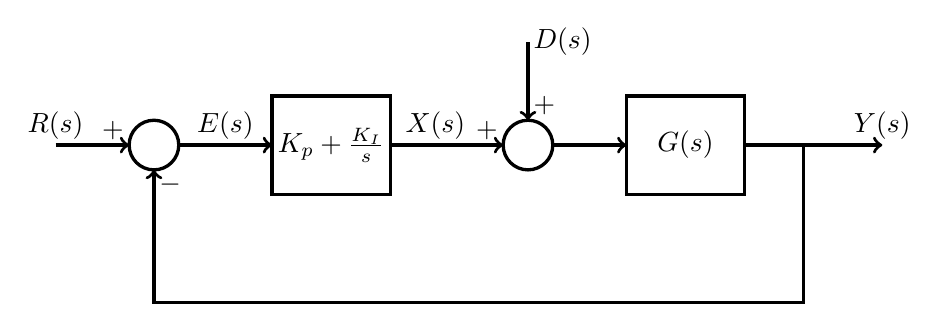
\begin{tikzpicture}[scale=1,inner sep=0pt,outer sep=0pt,very thick,
sysblock/.style={draw,rectangle,inner sep=2pt,minimum width=1.5cm,minimum height=1.25cm,very thick}]
\draw (1.25,0) node[draw,circle] (sum1) {$\rule{0pt}{18pt}$};
\draw (3.5,0) node[sysblock] (Kp) {$K_{p}+\frac{K_{I}}{s}$};
%\draw (5,0) node[draw,circle] (sum3) {$\rule{0pt}{18pt}$};
\draw (6,0) node[draw,circle] (sum2) {$\rule{0pt}{18pt}$};
\draw (8,0) node[sysblock] (G) {$G(s)$};
%\draw (8,-1.75) node[sysblock] (Kd) {$K_{d}s$};
\draw[->] (0,0) node[above=2pt] {$R(s)$} -- (sum1.180) node[above left=2pt] {$+$};
\draw[->] (sum1.0) --  node[above=2pt,pos=.5] {$E(s)$} (Kp);
%\draw[->] (Kp) -- (sum3.180) node[above left=2pt] {$+$};
\draw[->] (Kp.0) -- node[above=2pt,pos=.4] {$X(s)$}  (sum2.-180) node[above left=2pt] {$+$};
\draw[->] (sum2.0) -- (G);
\draw[->] (G) -- ++(2.5,0) node[above=2pt] {$Y(s)$};
%\draw[->] (G) ++(1.5,0) |- (Kd) -| (sum3.-90) node[below right=2pt] {$-$};
\draw[->] (G) ++(1.5,0) -- ++(0,-2) -| (sum1.-90) node[below right=2pt] {$-$};
\draw[<-] (sum2.90) node[above right=2pt] {$+$} -- ++(0,1) node[right=2pt] {$D(s)$};
\end{tikzpicture}
\end{center}
\end{frame}

\begin{example}\label{examp:PI} Let's return to the tank control problem, with a specified settling time of $\ts \leq 0.2$ s, but now $0$ steady state error for a unit step reference input. In order to meet these specifications with a proportional controller, we would need to apply infinite gain, so we instead turn to a PI control

\begin{frame}
\begin{center}
\input{Graphics/tankandvalvemeasPI}
\end{center}
\end{frame}
which has block diagram

\begin{frame}
\begin{center}
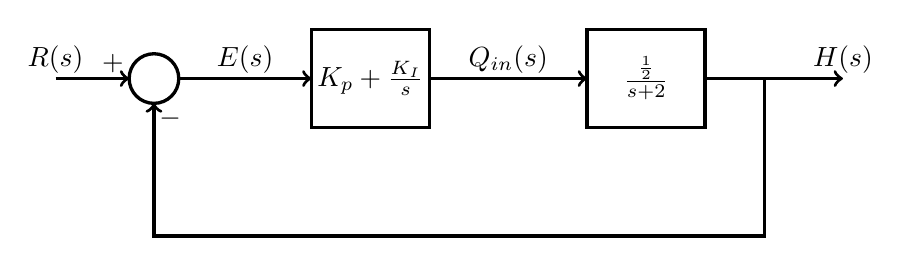
\begin{tikzpicture}[scale=1,inner sep=0pt,outer sep=0pt,very thick,
sysblock/.style={draw,rectangle,inner sep=2pt,minimum width=1.5cm,minimum height=1.25cm,very thick}]

\draw (1.25,0) node[draw,circle] (sum1) {$\rule{0pt}{18pt}$};
\draw (4,0) node[sysblock] (Kp) {$K_{p}+\frac{K_{I}}{s}$};
\draw (7.5,0) node[sysblock] (G) {$\frac{\frac{1}{2}}{s+2}$};

\draw[->] (0,0) node[above=2pt] {$R(s)$} -- (sum1.180) node[above left=2pt] {$+$};
\draw[->] (sum1.0) --  node[above=2pt,pos=.5] {$E(s)$} (Kp);
\draw[->] (Kp) -- node[above=2pt] {$Q_{in}(s)$} (G);
\draw[->] (G) -- ++(2.5,0) node[above=2pt] {$H(s)$};
\draw[->] (G) ++(1.5,0) -- ++(0,-2) -| (sum1.-90) node[below right=2pt] {$-$};
\end{tikzpicture}
\end{center}
\end{frame}
\begin{frame}
The closed loop transfer functions are
\begin{align*}
\frac{H(s)}{R(s)} &= \frac{\frac{K_{p}}{2}s+\frac{K_{I}}{2}}{s^2+\frac{4+K_{p}}{2}s+\frac{K_{I}}{2}}\\
\frac{E(s)}{R(s)} &= \frac{s^2+2s}{s^2+\frac{4+K_{p}}{2}s+\frac{K_{I}}{2}}
\end{align*}
Note that since $E(s)/R(s)$ has a zero at $s=0$, we automatically meet the steady state error specification, as
\[
e_{ss} = \lim_{s\rightarrow 0}s\frac{s^2+2s}{s^2+\frac{4+K_{p}}{2}s+\frac{K_{I}}{2}}\frac{1}{s} = 0
\]
We need only choose $K_{p}$ and $K_{I}$ to meet our settling time specification. 
\end{frame}
\begin{frame}
\mode<presentation>{\begin{center}
$\frac{H(s)}{R(s)} = \frac{\frac{K_{p}}{2}s+\frac{K_{I}}{2}}{s^2+\frac{4+K_{p}}{2}s+\frac{K_{I}}{2}}$
\end{center}}
Since $2\zeta\omega_{n} =\frac{4+K_{p}}{2}$, $\zeta\omega_{n} = 1+\frac{K_{p}}{4}$. Thus, we require
\[
\ts =\tseqtwo =  \frac{4.6}{1+\frac{K_{p}}{4}} \leq 0.2
\]
so we should choose
\[
K_{p}\geq 88
\]
$K_{I}$ can be chosen as desired. For example, we may wish to have a reasonable damping ratio.
\end{frame}
\begin{frame}
\mode<presentation>{\begin{center}
$\frac{H(s)}{R(s)} = \frac{\frac{K_{p}}{2}s+\frac{K_{I}}{2}}{s^2+\frac{4+K_{p}}{2}s+\frac{K_{I}}{2}}$
\end{center}}
From above,  $\zeta= \frac{1+\frac{K_{p}}{4}}{\omega_{n} }$, and from $\frac{H(s)}{R(s)}$, $\omega_{n} =\sqrt{\frac{K_{I}}{2}}$.  With $K_{p}=88$, 
\[
\zeta = \frac{(1+88/4)}{\omega_{n}} = \frac{23}{\sqrt{K_{I}/2}}
\]
So $K_{I} = 4232$ will give a damping ratio of $0.5$.
\end{frame}
\end{example}

}

\section{Using Simulink to Simulate Control Systems}
%\textcolor{red}{a lot of this part of the lecture can be removed in Fa'22 since we've had several lectures on Simulink already (especially the PD control example; maybe keep the PI?). }

In prior semesters, this lecture was the first in which Simulink was formally introduced. We have chosen to leave some of the Simulink content from prior semesters here for easy reference; for students who successfully applied P and PD control previously, the PI control section (Section \ref{sec:simulinkPI}) might be of most interest. 

\mode<all>{\mode<article>{\textsc{Matlab} has a graphical interface to run simulations of systems that are represented by block diagrams. While this is not as useful for creating simulation models of interconnected physical systems (in this case, another product, called Simscape is more useful) it is useful for creating simulations of systems with well defined input/output relationships, such as feedback control systems.

In addition to the example below, you can find a video introduction to Simulink at this link: \\ \hspace{.25in}\url{http://www.mathworks.com/videos/introduction-to-simulink-81623.html}\vspace{.1in}

You can start Simulink from the \textsc{Matlab} command line:\vspace{.1in}\\
\texttt{>> simulink} \vspace{.1in}\\
This will open up the following window, which give you access to all of the block elements in the Simulink Library}

\begin{frame}{Simulink Library}
\begin{center}
\begin{tikzpicture}
\draw (0,0) node {\includegraphics[height=2.8in]{Graphics/Simulink1}};
\draw (-4.15,3) node[circle,draw=red,very thick] {\rule{0pt}{6pt}};
\end{tikzpicture}
\end{center}
\end{frame}

To create a block diagram, we need to open up a new model window. This can be done by clicking on the new model icon (circled in red above). The result is a window that looks like the following:
\begin{frame}{Blank Simulink Model}
\begin{center}
\includegraphics[height=2.8in]{Graphics/Simulink2}
\end{center}
\end{frame}


\subsection{Simulink Example: PI Controller
\label{sec:simulinkPI}}
As an example, we will simulate the feedback control system for Example \ref{examp:PI}. We will grab blocks from the Simulink library and drag them over to the Simulink Model. The first block we need is a transfer function. There are two ways we can find a block. If we know which library it is in, we can click on that library in the ``Libraries'' window. So, for example, I know that transfer function blocks can be found in the ``Continuous''  library, and clicking on the word Continuous shows the blocks in that library. Note that the transfer function block is in the third column and third row.
\begin{frame}
\begin{center}
\includegraphics[height=2.8in]{Graphics/Simulink3}
\end{center}
\end{frame}

Alternately, we can search for the block using the search function. Type ``transfer'' into the search area (circled below) and you should see the list of blocks shown below. Note that the transfer function block is in the third column and first row.
\begin{frame}
\begin{center}
\begin{tikzpicture}
\draw (0,0) node {\includegraphics[height=2.8in]{Graphics/Simulink4}};
\draw (-2,2.95) node[ellipse,draw=red,minimum width=.6in,minimum height=.1in] {};
\end{tikzpicture}
\end{center}
\end{frame}

You can click on the transfer function block and drag it over to your model window. The model window should look like the following:
\begin{frame}
\begin{center}
\includegraphics[height=2.8in]{Graphics/Simulink5};
\end{center}
\end{frame}

Now do the following: In the library browser, click on the Continuous library, and drag the PID block to the model window, click on the Math Operations library and drag the sum to the model window, click on the Sources library and drag the step to the model window, and click on the Sinks library and drag the workspace block to the model window. Arrange the blocks is a line similar to the following:
\begin{frame}
\begin{center}
\includegraphics[height=2.8in]{Graphics/Simulink6};
\end{center}
\end{frame}

We can now connect up the blocks. Hover over the right side of the step block, in the region of the thick arrow head. The cursor should change to a plus sign. Click and drag the cursor over to the left side of the summer. An arrow should now connect these two blocks. Repeat this process until the model window is as follows: 
\begin{frame}
\begin{center}
\includegraphics[height=2.8in]{Graphics/Simulink7};
\end{center}
\end{frame}

We still need to connect the output of the transfer function block to the lower input of the summer. Do this by holding down the control key while clicking on the arrow that goes between the transfer function and the workspace block. Drag the cursor down and to the left, and then up until you hit the bottom of the summer. The result should look like the following:
\begin{frame}
\begin{center}
\includegraphics[height=2.8in]{Graphics/Simulink8};
\end{center}
\end{frame}

Now we can enter in the data for the blocks. Double click on the PID block, and a parameter window should open. Enter in the data so that the parameter window looks like the following: (Note that we are using $K_{p}$ and $K_{I}$ from Example 4). Now hit OK.
\begin{frame}
\begin{center}
\includegraphics[height=3.5in]{Graphics/Simulink9};
\end{center}
\end{frame}

Now double click on the transfer function block, and enter in the system transfer function for Example 4. Hit OK.
\begin{frame}
\begin{center}
\includegraphics[height=2.8in]{Graphics/Simulink10};
\end{center}
\end{frame}

The last thing we need to do is change the summer so that the bottom input is subtracted, not added. Double click on the summer, and change the last plus sign to a minus, as below. Hit OK.
\begin{frame}
\begin{center}
\includegraphics[height=2.8in]{Graphics/Simulink11};
\end{center}
\end{frame}

We are now ready to run the simulation. To choose the length of the simulation, enter the number of seconds in the box circled in red below. I have chosen 2 seconds. Then click on the green run button that is boxed in red below.
\begin{frame}
\begin{center}
\begin{tikzpicture}
\draw (0,0) node {\includegraphics[height=2.8in]{Graphics/Simulink12}};
\draw (3.2,2.6) node[ellipse,draw=red,minimum width=1.2in,minimum height=.1in] {};
\draw (-0.27,2.6) node[rectangle,draw=red,minimum width=.2in,minimum height=.2in] {};
\end{tikzpicture}
\end{center}
\end{frame}

Because we added a To Workspace block, the results of the simulation are in the variable \texttt{simout} in the Matlab workspace. The default is for this variable to be a \texttt{timeseries}, which is a structured variable that has several elements. Type \texttt{>> simout} at the command line to see the structure. We can plot the results either by typing \texttt{>> plot(simout)} or by typing \texttt{>> plot(simout.Time,simout.Data)}. This should result in the following plot:
\begin{frame}
\begin{center}
\includegraphics[height=2.8in]{Graphics/Simulink13};
\end{center}
\end{frame}

%\subsection{Simulink Example: PD Controller}
%
%For this example, we will implement a PD controller in Simulink. Let's take the block diagram for the PI controller in the previous example as our starting point. You might want to save this block diagram with a different name. 
%
%First, copy and paste the summer and PID control blocks, and connect them up as shown below. You can use command/control-I to flip a block direction, or right-click on the block and select rotate \& flip. 
%
%\begin{frame}
%\begin{center}
%\includegraphics[height=2.8in]{Graphics/PDsimulink1}
%\end{center}
%\end{frame}
%
%Click on the Transfer Fcn block and enter in the data for the motor system that is to be controlled.
%
%\begin{frame}
%\begin{center}
%\includegraphics[height=2.8in]{Graphics/PDsimulink2}
%\end{center}
%\end{frame}
%
%Click on the PID Controller block that will implement the proportional part of the controller, and enter in the proportional gain. (Actually, a simple gain block could also be used for this purpose.)
%
%\begin{frame}
%\begin{center}
%\includegraphics[height=3.5in]{Graphics/PDsimulink3}
%\end{center}
%\end{frame}
%
%Click on the PID Controller1 block that will implement the derivative part of the controller. Here we enter in the derivative gain, but we also have to choose a value for the filter coefficient \textsf{N}. We will select this to be 10 times the desired closed loop natural frequency. Since the desired closed loop $\omega_{n}$ is 22, enter 220 here.
%
%\begin{frame}
%\begin{center}
%\includegraphics[height=3.5in]{Graphics/PDsimulink4}
%\end{center}
%\end{frame}
%
%You can now run the simulation using the green arrow to start. 
%
%\begin{frame}
%\begin{center}
%\includegraphics[height=2.8in]{Graphics/PDsimulink5}
%\end{center}
%\end{frame}
%
%Type \texttt{>> plot(simout)} to get the following plot.
%
%\begin{frame}
%\begin{center}
%\includegraphics[height=2.8in]{Graphics/PDsimulink6}
%\end{center}
%\end{frame}
%
%Note that the rise time is 0.1s and the overshoot is 10\%, as desired.
%
%\textcolor{red}{Subsection ``What does the filter coefficient $N$ do?'' was moved to the PD control design lecture (\#13 in Fa'22)}}

%\section{Application Example}
%
%\noindent In Lectures \textcolor{red}{update references} we reviewed the wind turbine plant with pitch control input \(\beta\) and wind speed disturbance input \(u\) (Figure~\ref{fig:openloop}). If we place this wind turbine in a feedback control configuration with reference input \(\omega_{ref}\) and (preliminary) controller \(C(s) = 1\) as shown in Figure~\ref{fig:feedback}, what do we expect the steady-state error to a step reference input to be?
%\begin{figure}
%	\begin{center}
%		\includegraphics[width=6in]{graphics/Diagram}
%		\caption{Wind turbine plant (open loop) block diagram and associated transfer functions.}
%		\label{fig:openloop}
%	\end{center}
%\end{figure}
%
%\begin{figure}
%\begin{center}
%	\includegraphics[width=5in]{graphics/Diagram2}\\
%	\caption{Wind turbine plant with feedback control loop and disturbance input.}
%	\label{fig:feedback}
%\end{center}
%\end{figure}
%
%Referring to the Lecture \ReferenceSteadyStateErrorNumber \ article for the definition of System Type, we see that the feedback system is Type 0 (there are no pure integrators in \(C(s)G(s))\), which means that we expect a finite, nonzero steady-state error to a step reference input, and indeed we do observe such an error in Figure~\ref{fig:response} (note the $x$ axis: we've zoomed in on the last 50~s of the 300~s simulation to make it easier to see).
%\begin{figure}
%\begin{center}
%	\includegraphics[width=3in]{graphics/Diagram3}\\
%	\caption{Figure 2: Steady-state error to a unit step reference speed input.}
%	\label{fig:response}
%\end{center}
%\end{figure}
%
%We could predict the steady-state value of the error from the equation
%\begin{align*}
%e_{ss} &= \lim_{t \to \infty} e(t) = \frac{0.1}{1+K_p}\\
%K_p &= C(0)G(0)\\
%&= \frac{-21.201(6.509)}{(0.2867)(6.477)}\\
%&=-74.31\\
%&\Rightarrow e_{ss} = -0.0014
%\end{align*}
%
%\noindent Therefore, it is clear that the steady-state error should be quite small. (In fact, we need to run the simulation considerably longer, to more than 1000 s, before we reach ``steady state'' due to the slowness of the overall response).
%
%Including an integrator $\frac{1}{s}$ in the controller, for example as the integral portion of a PID controller, serves the purpose of creating a Type 1 system, which we understand has zero steady-state error to a step reference input. Simulation results verify this for sufficiently long simulations and appropriate choices of \(K_i\) and \(K_p\).
%
%Although we generally expect performance to improve when we increase the ``control authority'' (magnitudes of \(K_i\) and \(K_p\)), we should always ask whether increasing controller gains leads to the risk of instability. The next set of lectures on \textbf{Root Locus} helps us to answer that question.
%


\section{Lecture Highlights}
The primary takeaways from this article include
\begin{enumerate}
\setlength{\itemsep}{5pt}
\setlength{\parskip}{0pt}
\setlength{\parsep}{0pt}
\item \textcolor{red}{make sure to update list for Fa'22}
\item Proportional-Integral-Derivative (PID) control is commonly used in industry due to its straightforwardness and long history, which makes tuning the controller gains easier.
\item The proportional gain $K_p$ multiplies the error signal $e(t)$, the integral gain $K_I$ multiplies the integral of the error signal $\int{e(t)}$, and the derivative gain $K_D$ multiplies the derivative of the error signal $\dot{e}(t)$.
\item The PID gains can be computed to cause the closed-loop poles to lie within the allowable region to meet transient response specifications. However, since rules of thumb are not always precise, it is common for the system response not to meet specifications based on these initial calculations. Iterative tuning and checking response (for example, in Matlab) is common practice.
\item Simulink is a Matlab tool that enables additional flexibility for modeling more complex systems than may be possible in the Matlab command window. \textit{Note: a common point of confusion is the fact that Simulink models signals, such as the reference input, as blocks. This is opposed to the arrow designator for signals in standard block diagram conventions.}
\end{enumerate}


\section{Quiz Yourself}

\subsection{Questions}

\begin{enumerate}
\setlength{\itemsep}{5pt}
\setlength{\parskip}{0pt}
\setlength{\parsep}{0pt}
\item Consider a thermal system 
\begin{center}
\input{quizfigures/meloven2.tex}
\end{center}
that can be modeled with an equivalent thermal circuit (that can be treated just like an electrical circuit containing resistors, capacitors, a ``voltage'' source $v_{in}=T_a$, and a ``current'' source $i_{in}=K_h v_h$)
\begin{center}
\input{quizfigures/melcircuit2.tex}
\end{center}
You are going to design a PD controller for this system. You will measure the temperature reading of the thermocouple, compare it to a reference, and then use the PD controller to calculate the required voltage to the heater, $v_{h}$. The block diagram of your control system is as follows:
\begin{center}
\input{quizfigures/thermalcontrolblockdiag.tex}
\end{center}
where $C(s) = K_{p}+sK_{d}$, $G(s)=\frac{T_{2}(s)}{V_{h}(s)}$, and $F(s) = \frac{T_{2}(s)}{T_{a}(s)}\frac{1}{G(s)}$. The system parameters are $R_{v}=R=2$, $C=1$, $R_{T}=0.1$, $C_{T}=0.1$, $K_{h}=1$. 
\begin{enumerate}
\item Find $G(s)$ and $F(s)$. In each case, to find the transfer function from an input to an output signal, set all other sources equal to zero. In other words, to find $G(s)=\frac{T_{2}(s)}{V_{h}(s)}$, let $T_a(s)=0$ (short circuit). To find $F(s) = \frac{T_{2}(s)}{T_{a}(s)}\frac{1}{G(s)}$, let $V_h(s)=0$ (open circuit). 
\item Design a PD control so that a unit step command from $R(s)$ has rise time $t_{r}=0.1$s and overshoot $\%OS=10\%$. For this design you can assume $T_{a}(s)=0$. 
\item Confirm your design by finding the closed loop transfer function from $R(s)$ to $T_2(s)$ and using \textsc{Matlab} to plot the step response (See Lecture 12, section 4). You can assume $T_{a}(s)=0$. 
\item Find the steady state error for the unit step reference command.
\item Find the steady state error to a unit step change in the ambient temperature.  
\end{enumerate}
\end{enumerate}


\subsection{Solutions}
\begin{enumerate}
\setlength{\itemsep}{5pt}
\setlength{\parskip}{0pt}
\setlength{\parsep}{0pt}
\item \rule{0pt}{12pt}\\
\begin{center}
\includegraphics[width=6in]{quizfigures/2solna}\\
\includegraphics[width=6in]{quizfigures/2solnb}\\
\includegraphics[width=6in]{quizfigures/2solnc}
\end{center}
(c) We want to simulate the  configuration
\begin{center}
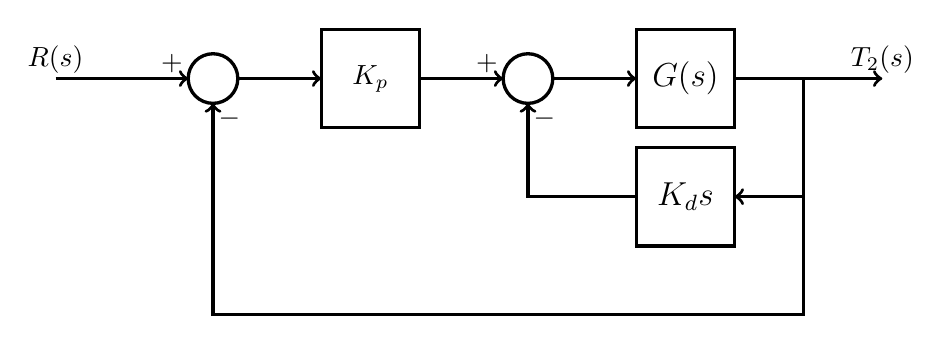
\begin{tikzpicture}[scale=1,inner sep=0pt,outer sep=0pt,very thick,
sysblock/.style={draw,rectangle,inner sep=2pt,minimum width=1.25cm,minimum height=1.25cm,very thick}]
\draw (2,0) node[draw,circle] (sum1) {$\rule{0pt}{18pt}$};
\draw (4,0) node[sysblock] (Kp) {$\large K_p$};
\draw (6,0) node[draw,circle] (sum2) {$\rule{0pt}{18pt}$};
\draw (8,0) node[sysblock] (G) {\large $G(s)$};
\draw (8,-1.5) node[sysblock] (Kd) {\large $K_{d}s$};
\draw[->] (0,0) node[above=2pt] {$R(s)$} -- (sum1.180) node[above left=2pt] {$+$};
\draw[->] (sum1.0) --  (Kp);
\draw[->] (Kp) -- (sum2.180) node[above left=2pt] {$+$};

%\draw[<-] (sum2.90) node[above right=2pt] {$+$} -- (F.-90);
%\draw[<-] (F.90) -- ++(0,1) node[right=2pt] {$T_{a}(s)$};
\draw[->] (sum2) -- (G);
%\draw[->] (Kp.0) -- (G.180);
\draw[->] (G) -- ++(2.5,0) node[above=2pt] {$T_{2}(s)$};
\draw[->] (G) ++(1.5,0) -- ++(0,-1.5) -- (Kd.0);
\draw[->] (G) ++(1.5,0) -- ++(0,-3) -| (sum1.-90) node[below right=2pt] {$-$};
\draw[->] (Kd.180) -| (sum2.-90) node[below right=2pt] {$-$};
\end{tikzpicture}

\end{center}
This has closed loop system
\[
\frac{T_{2}(s)}{R(s)}=T(s)=\frac{100}{s^{2}+(111+100K_d)s+100(1+K_p)},
\]
and using the code
\texttt{\rule{0pt}{0pt}\\
Kp=3.84;\\
Kd=-0.85;\\
\% Configuration \#2
figure(1)\\
T = tf(100*Kp,[1 111+100*Kd 100*(1+Kp)])\\
step(T)}\\
we get the following plot:
\begin{center}
\includegraphics[width=4in]{quizfigures/prob3_2}
\end{center}
\begin{center}
\includegraphics[width=6in]{quizfigures/2solnd}\\
\includegraphics[width=6in]{quizfigures/2solne}
\end{center}
\end{enumerate}

\section{Resources}

\subsection{Books}


\begin{itemize}
\item Gene F. Franklin, J. David Powell and Abbas Emami-Naeini,  {\em Feedback Control of Dynamic Systems}, Pearson
\begin{itemize}
\item 6th and 7th edition: Section 4.3
\end{itemize}
\end{itemize}


\subsection{Web resources}
The following are web resources concerning PID controllers. If you find something else on the web that is useful, or if you find a link that no longer works, please inform your instructor!


\begin{itemize}
\item \url{http://ctms.engin.umich.edu/CTMS/index.php?example=Introduction&section=ControlPID} - An interactive tutorial of PID controllers that is designed to be covered while you have access to \textsc{Matlab}.
\item \url{https://www.youtube.com/watch?v=XfAt6hNV8XM} A 13 minute video with some examples of PID control.


\end{itemize}



\section{Appendix: Implementing a PID controller on a microcontroller}

A PID controller is easily implemented on a micro-controller, and only requires a few lines of code. The main issue is that a micro-controller is a discrete time system, in that it can only read or write in discrete times. Thus, we need to find discrete time approximations to the integral and derivative. The basic functionality is as follows:

\textsf{\\
Set \texttt{Kp}, \texttt{Ke}, \texttt{Ki} to PID control gains\\
Set \texttt{I := 0}\\
Set \texttt{e\_past := 0}\\
Set \texttt{Ts := 0}\\
Set \texttt{Tc :=} current time\\
\\
Loop:\\
\rule{0pt}{0pt}\hspace{.1in}Read \texttt{r}, current value of reference variable (supplied by the user, probably input using a user interface)\\
\rule{0pt}{0pt}\hspace{.1in}Read \texttt{y}, current value of system output \\
\rule{0pt}{0pt}\hspace{.1in}Calculate \texttt{e := r-y}, the error\\
\rule{0pt}{0pt}\hspace{.1in}{\color{red} If \texttt{Ts>0}, \\
\rule{0pt}{0pt}\hspace{.2in}Calculate \texttt{D := (e - e\_past)/Ts}, Set \texttt{e\_past := e}, \\
\rule{0pt}{0pt}\hspace{.1in}else\\
\rule{0pt}{0pt}\hspace{.2in}Set \texttt{D := 0}}\\
\rule{0pt}{0pt}\hspace{.1in}{\color{violet} Calculate \texttt{I := I + Ts*e}}\\
\rule{0pt}{0pt}\hspace{.1in}{\color{blue} Calculate controller output \texttt{u = Kp*e + Ki*I + Kd*D}} \\
\rule{0pt}{0pt}\hspace{.1in}Set output to \texttt{u} (for example, setting a voltage to \texttt{u} using a digital to analog element)\\
\rule{0pt}{0pt}\hspace{.1in}Set \texttt{Ts := } current time minus \texttt{Tc}\\
\rule{0pt}{0pt}\hspace{.1in}Set \texttt{Tc := } current time\\
End Loop:
}

The blue line is where the PID control output is calculated. The first time through the loop, only the proportional term will be utilized, as two samples are necessary to calculate the derivative, and the integral of a single sample is zero.
In the next subsections, we explain the red and purple lines, which are the discrete time approximations to derivative and integral. 

\subsection{Approximation to a Derivative}

Given a function $e(t)$, the definition of derivative is
\[
\frac{de}{dt} = \lim_{h\rightarrow  0} \frac{e(t) - e(t-h)}{h}
\]
In the micro-controller, we can only calculate $e(t)$ at discrete times as we go through the loop. Our approximation will be to take $h$ to be this cycle time, which is the variable \texttt{Ts}. Thus
\[
{\color{red} \frac{de}{dt} \approx \frac{e(t) - e(t-\texttt{Ts})}{\texttt{Ts}}}
\] 
Note that $e(t-\texttt{Ts})$ is saved in the variable \texttt{e\_past}.
\subsection{Approximation to an Integral}

The integral of a function is the area under the graph. When we only get discrete samples of the function we can approximate the area using rectangles whose width is the sample time, and height are the samples. This is illustrated below, where the sample time is fixed to $T_{s}$ seconds.

\begin{center}
\includegraphics[width=4in]{Graphics/backwardrectangle}
\end{center}

As an equation, we can define the approximation as follows: Let $i(t)$ be the function that is the integral of $e(t)$ from $0$ to $t$. The exact calculation of $i(t)$ is
\[
i(t) = \int_{0}^{t} e(\tau)d\tau.
\]
Suppose we want to calculate $i(t)$ at sample $N$, so that  $t=NT_{s}$. The approximation is 
\[
i(t) = i(NT_{s}) \approx \sum_{k=1}^{N} e(kT_{s})T_{s}.
\]
Since we keep adding new terms as $t$ increases, we can also calculate this recursively as
\[
{\color{purple} i(NT_{s}) = i((N-1)T_{s}) + e(NT_{s})T_{s}.}
\]


\subsection{Anti-windup - accounting for actuator saturation}

It is very common for the control output $u(t)$ to be only valid over a finite range. For example, if you have a D/A board that can only supply a maximum of $\pm 10$ volts, then $u$ can only lie between -10 and 10. Even if we calculate a larger value of \texttt{u}, only $10$ volts will be delivered. In this case, the output is {\em saturated}. Output saturation can have detrimental effects on the integral control element, as the error will be larger than expected, causing the integral term to {\em wind-up}, or count up to a very large value.  This can be counteracted by limiting the integral term when saturation occurs. The modified code that includes anti-windup is as follows:

\textsf{\\
Set \texttt{Kp}, \texttt{Ke}, \texttt{Ki} to PID control gains\\
{\color{cyan} Set \texttt{umax} to maximum control magnitude}\\
Set \texttt{I := 0}\\
Set \texttt{e\_past := 0}\\
Set \texttt{Ts := 0}\\
Set \texttt{Tc :=} current time\\
\\
Loop:\\
\rule{0pt}{0pt}\hspace{.1in}Read \texttt{r}, current value of reference variable (supplied by the user, probably input using a user interface)\\
\rule{0pt}{0pt}\hspace{.1in}Read \texttt{y}, current value of system output \\
\rule{0pt}{0pt}\hspace{.1in}Calculate \texttt{e := r-y}, the error\\
\rule{0pt}{0pt}\hspace{.1in}{\color{red} If \texttt{Ts>0}, \\
\rule{0pt}{0pt}\hspace{.2in}Calculate \texttt{D := (e - e\_past)/Ts}, Set \texttt{e\_past := e}, \\
\rule{0pt}{0pt}\hspace{.1in}else\\
\rule{0pt}{0pt}\hspace{.2in}Set \texttt{D := 0}}\\\rule{0pt}{0pt}\hspace{.1in}{\color{violet} Calculate \texttt{I := I + Ts*e}}\\
\rule{0pt}{0pt}\hspace{.1in}{\color{blue} Calculate controller output \texttt{u = Kp*e + Ki*I + Kd*D}} \\
\rule{0pt}{0pt}\hspace{.1in}{\color{cyan} If \texttt{abs(u)>umax},  \\
\rule{0pt}{0pt}\hspace{.2in}\texttt{u := sgn(u)*umax} \quad (saturate output)\\
\rule{0pt}{0pt}\hspace{.2in}\texttt{I := I - Ts*e} \quad (undo integration)}\\ 
\rule{0pt}{0pt}\hspace{.1in}Set output to \texttt{u}  \quad (for example, setting a voltage to \texttt{u} using a digital to analog element)\\
\rule{0pt}{0pt}\hspace{.1in}Set \texttt{Ts := } current time minus \texttt{Tc}\\
\rule{0pt}{0pt}\hspace{.1in}Set \texttt{Tc := } current time\\
End Loop:\\
}

Note that the new lines are in cyan.






\end{document}


